\documentclass[letterpaper,11pt]{article}

\usepackage{geometry}
\usepackage{pslatex}
\usepackage{fancyhdr}
\usepackage{graphicx}
\usepackage{setspace}
\usepackage{amsmath, amssymb}
\usepackage{hyperref}
\usepackage{amsfonts}

\geometry{ margin = 1.0in }

\pagestyle{fancy}
\lhead{{\bf CMPSC 431W}}
\chead{{\bf Database Management System}}
\rhead{{\bf \today}}

\setlength\parindent{0em}
\setlength\parskip{8pt}

\newcommand{\Paragraph}[1]{~\vspace*{-0.7\baselineskip}\\{\bf #1}}



\begin{document}

\begin{center}
	{\LARGE \bf Assignment 5 Solution}
	
	{\large
	Name: Yanjun Chen, PSU ID: yfc5289}
\end{center}

\section*{Part I: Problem 1}
\Paragraph{
	Set up the table, its schema, cardinality just use the question statement in problem 2: \\
	Schema: Student\((\)\underline{SID}, firstname, lastname, GPA, program\()\)\\
	With the following facts: \\
	1. this table contains more than 1 million records; \\
	2. \((\)firstname, lastname\()\) is a candidate key for this table; \\
	3. students are evenly distributed across 20 programs; \\
	4. GPA of all the students form a normal distribution around 3.0 with a standard deviation of 1.0. 
	Case where answering a database query with an index is strictly slower than scanning through the whole file: \\
	Use the non-cluster Btree, put index on \((\)program, GPA\()\), find all the lastname for students with specific GPA 
	range from all the programs. \\


}

\section*{Part I: Problem 2}
\Paragraph{1. }
\begin{verbatim}
	CREATE INDEX IDX1 ON Student(lastname) USING HASH;
\end{verbatim}

\Paragraph{2.}
\begin{verbatim}
	CREATE INDEX IDX2 ON Student(GPA) USING BTREE;
\end{verbatim}

\Paragraph{3. \\
	\underline{Notes for this problem:} each answer query also with the example: \\
	1. single program point lookup: find the specific program. such as "CS". \\
	2. single program range: find the list of programs with specific index range as they got "index on". \\
	3. point lookup on both: find the records of students who got program in "CS" and with specific GPA 4.0. \\
	4. range on both: find the records of students with given program range and given GPA range. \\
	5. range on program and point lookup on GPA: find the records of student in range of progran with given GPA, such as 4.0 GPA. \\
	6. point lookup on program and range on GPA: find the records of students in specific program with given range of GPA. 

}

\newpage
\section*{Part I: Problem 2}
\Paragraph{4.}
\begin{verbatim}
	CREATE INDEX IDX1 ON Student(program, GPA) USING BTREE
\end{verbatim}
We need BTREE for GPA to accelerate the requirement \((a)\) and \((c)\). \\
\begin{verbatim}
	CREATE INDEX IDX2 ON Student(firstname, lastname) USING HASH
\end{verbatim}
The full name is just a simple point look up, so HASH makes more sense here. 


\section*{Part II: Problem 1}
\begin{figure}[h]
    \centering
    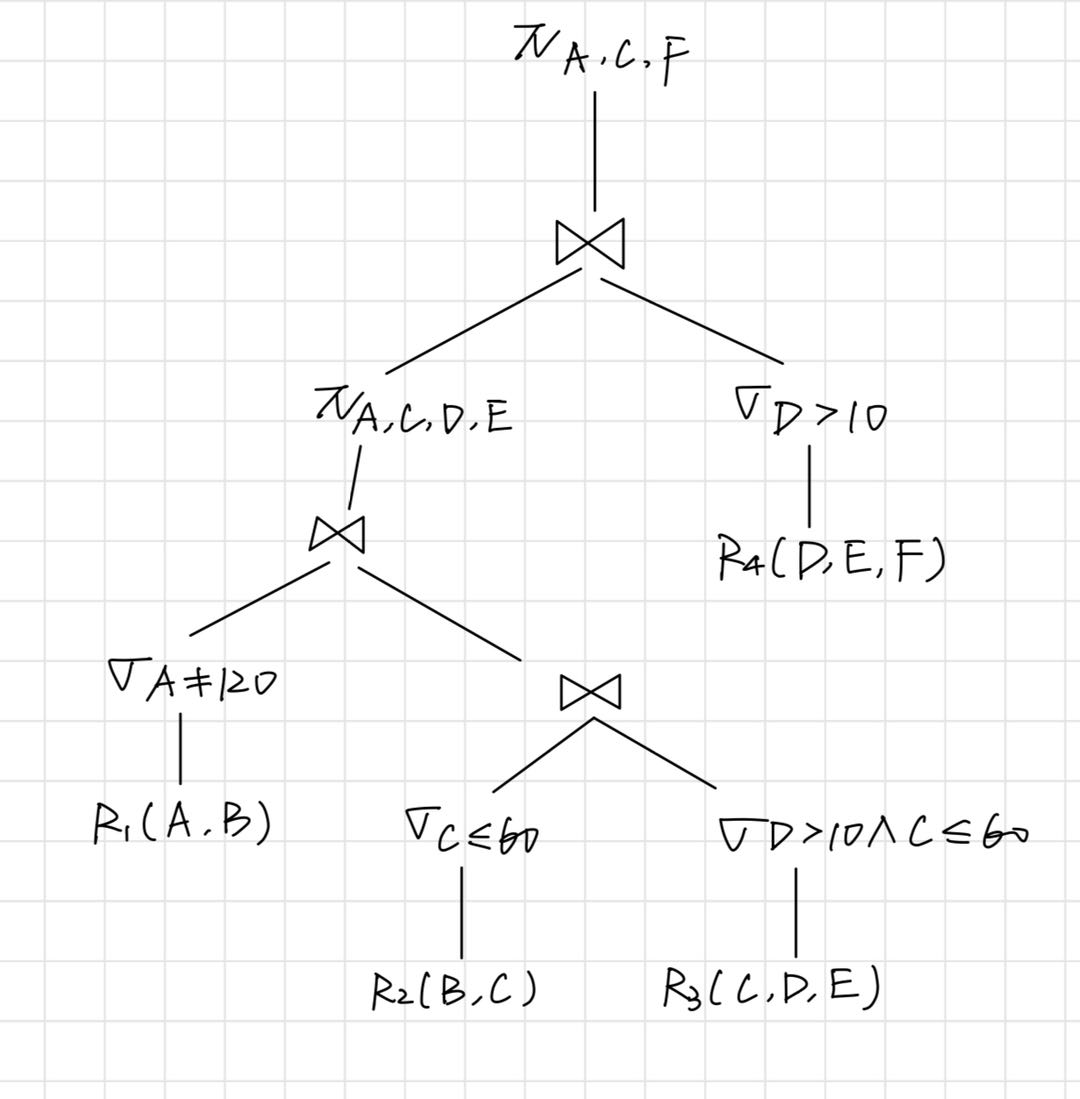
\includegraphics[width=0.7\textwidth]{p2-1.jpg}
\end{figure}

\newpage
\section*{Part II: Problem 2}
\(P(R_1) = 50000/200 = 250\); \(P(R_2) = 30000/200 = 150\); \(P(R_3) = 10000/200 = 50\);\\
\(P(R_1 \Join R_2) = 10000/200 = 50; P(R_1 \Join R_3) = 4000/200 = 20; P(R_2 \Join R_3) = 1000/200 = 5\);\\
\(P(R_1 \Join R_2 \Join R_3) = 500/200 = 2.5\); 



\Paragraph{1. \\
	cost = \(P(R_1) + \frac{P(R_1) \cdot P(R_3)}{B - 1} + OUT(R_1 \Join R_3) + 
	P(R_1 \Join R_3) + \frac{P(R_1 \Join R_3) \cdot P(R_2)}{B - 1} + OUT(R_1 \Join R_2 \Join R_3)\) \\
	= 250 + 1250 + 40 +300 + 2.5 \\ 
	= 1842.5 = 1843\\

}

\Paragraph{2. every physical cases \\
	1. \(R_1 \Join R_2\) first, then \(R_3\):\\
	cost = \(P(R_1) + \frac{P(R_1) \cdot P(R_2)}{B - 1} + OUT(R_1 \Join R_2) + 
	P(R_1 \Join R_2) + \frac{P(R_1 \Join R_2) \cdot P(R_3)}{B - 1} + OUT(R_1 \Join R_2 \Join R_3)\) \\
	= 250 + 3750 + 50 + 50 + 250 + 2.5 \\
	= 4352.5 = 4353\\

	2. \(R_2 \Join R_1\) first, then \(R_3\):\\
	cost = \(P(R_2) + \frac{P(R_1) \cdot P(R_2)}{B - 1} + OUT(R_1 \Join R_2) + 
	P(R_1 \Join R_2) + \frac{P(R_1 \Join R_2) \cdot P(R_3)}{B - 1} + OUT(R_1 \Join R_2 \Join R_3)\) \\
	= 150 + 3750 + 50 + 50 + 250 + 2.5 \\
	= 4252.5 = 4253\\

	3. \(R_1 \Join R_3\) first, then \(R_2\)
	cost = \(P(R_1) + \frac{P(R_1) \cdot P(R_3)}{B - 1} + OUT(R_1 \Join R_3) + 
	P(R_1 \Join R_3) + \frac{P(R_1 \Join R_3) \cdot P(R_2)}{B - 1} + OUT(R_1 \Join R_2 \Join R_3)\) \\
	= 250 + 1250 + 40 +300 + 2.5 \\ 
	= 1842.5 = 1843\\


	4. \(R_3 \Join R_1\) first, then \(R_2\): \\
	cost = \(P(R_3) + \frac{P(R_1) \cdot P(R_3)}{B - 1} + OUT(R_1 \Join R_3) + 
	P(R_1 \Join R_3) + \frac{P(R_1 \Join R_3) \cdot P(R_2)}{B - 1} + OUT(R_1 \Join R_2 \Join R_3)\) \\
	= 50 + 1250 + 40 +300 + 2.5 \\ 
	= 1642.5 = 1643\\

	5. \(R_2 \Join R_3\) first, then \(R_1\): \\
	cost = \(P(R_2) + \frac{P(R_2) \cdot P(R_3)}{B - 1} + OUT(R_2 \Join R_3) + 
	P(R_2 \Join R_3) + \frac{P(R_2 \Join R_3) \cdot P(R_1)}{B - 1} + OUT(R_1 \Join R_2 \Join R_3)\) \\
	= 150 + 750 + 5 + 5 + 125 + 2.5\\
	= 1037.5 = 1038\\

	6. \(R_3 \Join R_2\) first, then \(R_1\): \\
	cost = \(P(R_2) + \frac{P(R_2) \cdot P(R_3)}{B - 1} + OUT(R_2 \Join R_3) + 
	P(R_2 \Join R_3) + \frac{P(R_2 \Join R_3) \cdot P(R_1)}{B - 1} + OUT(R_1 \Join R_2 \Join R_3)\) \\
	= 50 + 750 + 5 + 5 + 125 + 2.5\\
	= 937.5 = 938\\

	Because \(938 < 1038 < 1643 < 1843 < 4253 < 4353\), \(R_3 \Join R_2\) first, then \(R_1\) is the best plan. 
	

}






\end{document}



